%%%%%%%%%%%%%%%%%%%%%%%%%%%%%%%%%%%%%%%%%%%%%%%%%%%%%%%%%%%%%%%%%%%%%%%%%%%%%%%%%%%%%%%%
\chapter{Loop models: A perturbation theory study of Kitaev models}
\label{appendix:LoopModels}

\newcommand{\note}[1]{\textbf{#1}}

%%%%%%%%%%%%%%%%%%%%%%%%%%%%%%%%%%%%%%%%%%%%%%%%%%%%%%%%%%%%%%%%%%%%%%%%%%%%%%%%%%%%%%%%
%
%
In this appendix are reported the results of a study of the Kitaev Hamiltonian deep in the gapped phase on a number of lattices.
For each lattice an effective loop model is derived via a perturbative expansion in the exchange couplings $J_x,~J_y \ll J_z$.
As this study was never finished, the level of detail varies for each lattice.
This appendix should be thought of as reference point for anyone wishing to further explore this topic.

Following the approach of Reference~\cite{KitaevAoP2006}, the Kitaev Hamiltonian is rewritten as
%
\begin{equation}
	H = H_0 + V,
\end{equation}
%
where
%
\begin{equation}
	H_0 = -J_z \sum_{z \rm-bonds} \sigma_j^z \sigma_k^z
\end{equation}
%
and
%
\begin{equation}
	V = -J_x \sum_{x \rm-bonds} \sigma_j^x \sigma_k^x - J_y \sum_{y \rm-bonds} \sigma_j^y \sigma_k^y.
	\label{eq:appendix1_PotentialTerm}
\end{equation}
%
For concreteness, consider $J_z > 0$ in the following.
The ground state of $H_0$ is given by a configuration for which all pairs of spins connected by a $z$-link are aligned.
There remains, however, an extensive ground state degeneracy as their common direction is not fixed by $H_0$.
The ground state energy is $E_0 = -N J_z$, where $N$ is the number of $z$-bonds, \ie, half the number of spins.

In this degenerate ground state subspace, one may define a lattice of effective spins by regarding each pair of physical spins which are connected by a $z$-bond as a single effective spin.
The operator $\Upsilon:\mathcal{L}_{\rm eff} \rightarrow \mathcal{L}$ which maps the Hilbert space of effective spins onto the ground state subspace of $H_0$ is defined by $\Upsilon:\ket{m} \mapsto \ket{m m}$, where $m =\, \uparrow$ or $m =\, \downarrow$.

The goal is to find an effective Hamiltonian which acts in the space of effective spins $\mathcal{L}_{\rm eff}$.
Writing the Green's function $\Upsilon\dag (E - H)^{-1} \Upsilon$ in terms of the self-energy as $(E - E_0 - \Sigma(E))^{-1}$ and neglecting the dependence of the self-energy $\Sigma(E)$ on $E$ for $E \approx E_0$, one may define an effective Hamiltonian as $H_{\rm eff} = E_0 + \Sigma(E_0)$.

The task now is to solve for the self-energy
%
\begin{equation}
	\Sigma(E) = \Upsilon\dag (V + V G'_0(E) V + V G'_0(E) V G'_0(E) V + \dots) \Upsilon,
	\label{eq:self-energy}
\end{equation}
%
where $G'_0(E)$ is the Green's function of the unperturbed Hamiltonian $H_0$, with the prime indicating that it vanishes when acting on ground states.
Setting $E = E_0$, one may now compute $H_{\rm eff} = E_0 + \Sigma(E_0)$ order by order.

In the following sections, this effective Hamiltonian is found for a number of tricoordinated lattices.
Some of the general ideas are first explored in the simplest case of the honeycomb lattice (6,3) before being applied to the three-dimensional lattices in the latter sections.


%
%
%%%%%%%%%%%%%%%%%%%%%%%%%%%%%%%%%%%%%%%%%%%%%%%%%%%%%%%%%%%%%%%%%%%%%%%%%%%%%%%%%%%%%%%%
\section{Lattice (6,3)}
\label{appendix:LoopModels_6_3}
%%%%%%%%%%%%%%%%%%%%%%%%%%%%%%%%%%%%%%%%%%%%%%%%%%%%%%%%%%%%%%%%%%%%%%%%%%%%%%%%%%%%%%%%
%
%
It is clear that all odd-order contributions to the self-energy must vanish as they map to states outside of the ground state subspace.
The first non-vanishing contribution arrives at second order as
%
\begin{equation}
	\Sigma^{(2)}(E_0) = -\sum_{x \rm-links} \frac{J_x^2}{4 J_z} - \sum_{y \rm-links} \frac{J_y^2}{4 J_z} = -N \frac{J_x^2 + J_y^2}{4 J_z}.
\end{equation}
%
One can see that each term $\sigma_j^x \sigma_k^x$ or $\sigma_j^y \sigma_k^y$ in the first $V$ acts to flip a pair of spins with an energy cost of $4 J_z$.
The second $V$ then acts to flip those spins back, leaving the state unaltered and resulting in a term proportional to the identity operator.

The first \textit{non}-constant terms arrive at fourth order.
The honeycomb lattice is comprised of hexagonal plaquettes, each of which includes four effective spins connected by two $x$- and two $y$-bonds (see Figure~\ref{fig:appendix1_Honeycomb}).
Thus, at fourth order, it is possible to act on all $x$- and $y$-bonds in the plaquette, resulting in an operator which maps from one degenerate ground state to another.
There are $4! = 24$ such terms, each of which is proportional to the loop operator $\tau_4^z \tau_3^y \tau_2^z \tau_1^y$, where $\tau_j^\gamma$ are Pauli matrices acting on the effective spins (see Figure~\ref{fig:appendix1_Honeycomb}~(b)).
The structure of the loop operator can be surmised from the way products of two physical spin operators act in the space of effective spins,
%
\begin{align}
	\Upsilon\dag \sigma_{j,\mu}^x \sigma_{j,\mu}^y \Upsilon \ket{m_j} &= i m_j \ket{m_j} = i \tau_j^z \ket{m_j} \nonumber\\
	\Upsilon\dag \sigma_{j,\mu}^x \sigma_{j,\nu}^y \Upsilon \ket{m_j} &= i m_j \ket{-m_j} = \tau_j^y \ket{m_j} \nonumber\\
	\Upsilon\dag \sigma_{j,\mu}^x \sigma_{j,\nu}^x \Upsilon \ket{m_j} &= \ket{-m_j} = \tau_j^x \ket{m_j} \nonumber\\
	\Upsilon\dag \sigma_{j,\mu}^y \sigma_{j,\nu}^y \Upsilon \ket{m_j} &= -\ket{-m_j} = -\tau_j^x \ket{m_j},
	\label{eq:appendix1_SpinRules}
\end{align}
%
where $j$ indexes the effective spin (or $z$-bond), while $\mu$ and $\nu$ index the physical spins connected by $z$-bond $j$ (see Figure~\ref{fig:appendix1_Honeycomb}~(a)) and are understood to be strictly not equal.

The numerical prefactor for each of these loop operator terms corresponds to how many $z$-bonds are virtually excited after each successive application of the operator $V$.
This, as well as the overall sign of the individual term, depends on the order in which the link operators $\sigma_j^\gamma \sigma_k^\gamma$ are applied.
Of the 24 total terms, twelve have prefactor $-\frac{J_x^2 J_y^2}{64 J_z^3}$, four have prefactor $+\frac{J_x^2 J_y^2}{64 J_z^3}$ and eight have prefactor $+\frac{J_x^2 J_y^2}{128 J_z^3}$ yielding a fourth-order contribution to the self-energy of
%
\begin{equation}
	\Sigma^{(4)}(E_0) = {\rm const} - \frac{J_x^2 J_y^2}{16 J_z^3} \sum_{p} \tau_1^z \tau_2^y \tau_3^z \tau_4^y,
	\label{eq:honeycomb-loop-term}
\end{equation}
%
where the summation runs over all plaquettes and the effective spin operators are understood to act on the effective spins of plaquette $p$ (as pictured in Figure~\ref{fig:appendix1_Honeycomb}).
All plaquettes in the honeycomb lattice are equivalent in the sense that all terms in the summation in Eq.~\eqref{eq:honeycomb-loop-term} are of the same form.
At this stage, one may apply a unitary transformation to the effective Hamiltonian to yield the well known toric code model~\cite{KitaevAoP2003,KitaevAoP2006}.
%
\begin{figure}[tb]
	\centering
	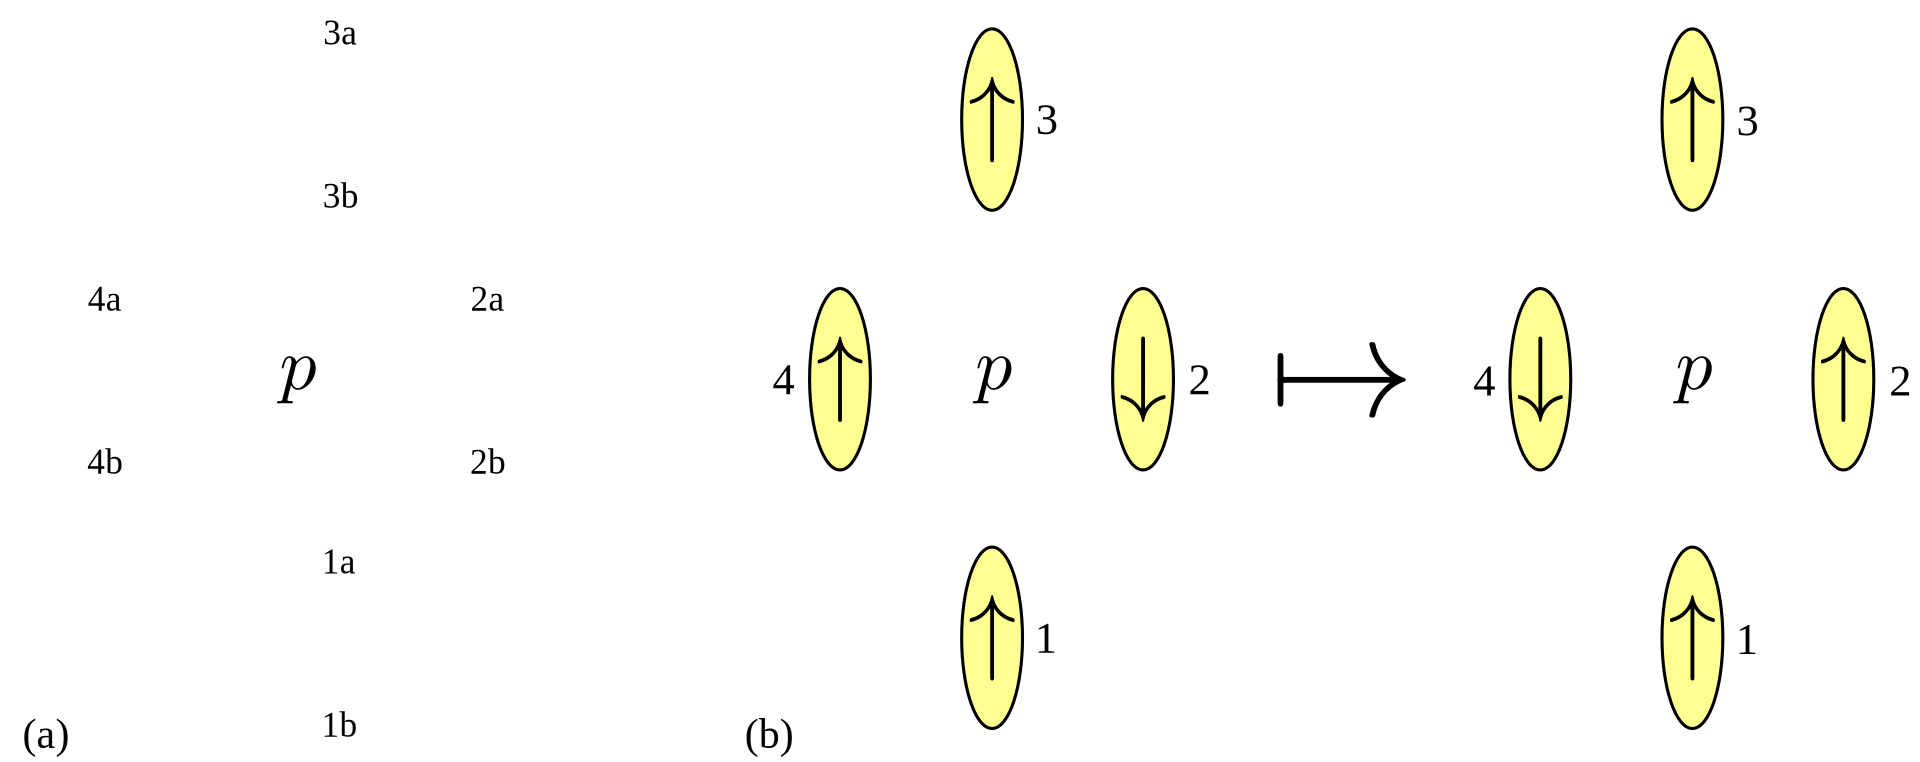
\includegraphics[width=\linewidth]{./appendixLoopModels/honeycomb.pdf}
	\caption{(a) Numbering scheme for the physical spin operators of a plaquette $p$. (b) Example of how a loop operator acts on the effective spins of a plaquette $p$.}
	\label{fig:appendix1_Honeycomb}
\end{figure}
%


%
%
%%%%%%%%%%%%%%%%%%%%%%%%%%%%%%%%%%%%%%%%%%%%%%%%%%%%%%%%%%%%%%%%%%%%%%%%%%%%%%%%%%%%%%%%
\section{Lattice (10,3)b}
\label{appendix:LoopModels_10_3b}
%%%%%%%%%%%%%%%%%%%%%%%%%%%%%%%%%%%%%%%%%%%%%%%%%%%%%%%%%%%%%%%%%%%%%%%%%%%%%%%%%%%%%%%%
%
%
%%%%%%%%%%%%%%%%%%%%%%%%%%%%%%%%%%%%%%%%%%%%%%%%%%%%%%%%%%%%%%%%%%%%%%%%%%%%%%%%%%%%%%%%
\subsubsection{Effective Hamiltonian}
%%%%%%%%%%%%%%%%%%%%%%%%%%%%%%%%%%%%%%%%%%%%%%%%%%%%%%%%%%%%%%%%%%%%%%%%%%%%%%%%%%%%%%%%
%
%
As before, all odd-order contributions to the self-energy vanish as they map to states outside of the ground state subspace.
While there are non-zero contributions to the self-energy which are proportional to the identity operator at second and fourth order, the first non-trivial contribution arrives at sixth order in perturbation theory.

The lattice (10,3)b is composed entirely of loops of length 10.
There are four such loops per unit cell, each of which involves six effective spins and either four $x$-bonds and two $y$-bonds (see Figures~\ref{fig:appendix1_10_3b}~(a) and (b)) or two $x$-bonds and four $y$-bonds (see Figures~\ref{fig:appendix1_10_3b}~(c) and (d)).

Each plaquette corresponds to $6! = 720$ terms, each of which is proportional to a loop operator which acts on the effective spins as described in Eq.~\eqref{eq:appendix1_SpinRules}.
The sixth-order contribution to the self-energy is
%
\begin{align}
	\Sigma^{(6)}(E_0) = &{\,\rm const} - \frac{7 J_x^4 J_y^2}{256 J_z^5} \left( \sum_{p_a} \tau_1^z \tau_2^y \tau_3^x \tau_4^z \tau_4^y \tau_6^x + \sum_{p_b} \tau_1^y \tau_6^x \tau_5^z \tau_7^y \tau_8^x \tau_{10}^z \right) \nonumber\\
	&- \frac{7 J_x^2 J_y^4}{256 J_z^5} \left( \sum_{p_c} \tau_1^x \tau_2^y \tau_3^z \tau_9^x \tau_8^y \tau_{10}^z + \sum_{p_d} \tau_3^y \tau_4^z \tau_5^x \tau_7^y \tau_8^z \tau_9^x \right),
\end{align}
%
where each summation is over all plaquettes of a given type, \ie, $p_a$ corresponds to the plaquette type shown in Figure~\ref{fig:appendix1_10_3b}~(a) and similarly for the remaining three summations.
%
\begin{figure}[tb]
	\centering
	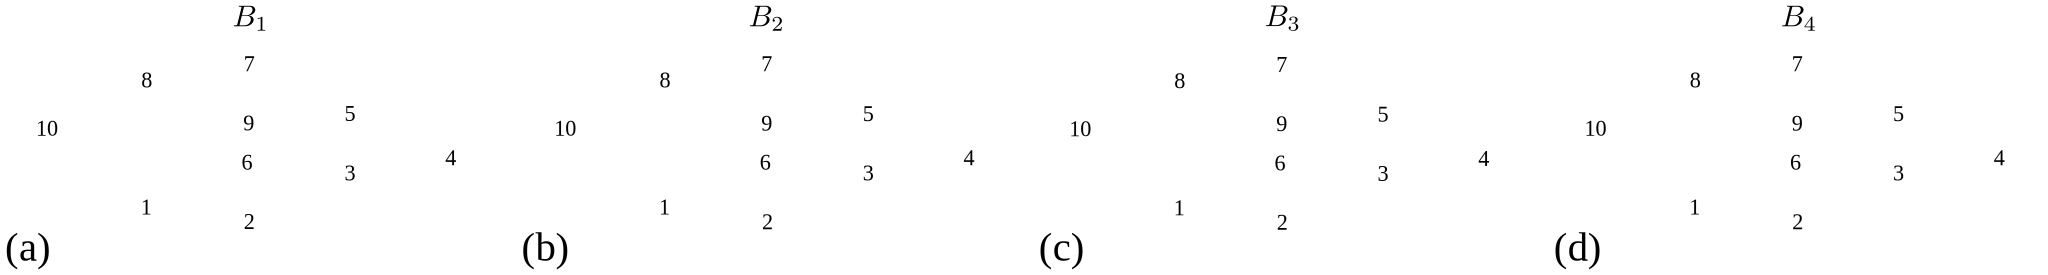
\includegraphics[width=\linewidth]{./appendixLoopModels/hyperhoneycomb.pdf}
	\caption{Four loops of length 10 in lattice (10,3)b become loops of length 6 in the lattice of effective spins.}
	\label{fig:appendix1_10_3b}
\end{figure}
%

Following the work of Reference~\cite{MandalPRB2014}, the effective Hamiltonian will now be rewritten in a more succinct form.
There are two effective spins per unit cell at positions
%
\begin{equation}
	\br_1 = \left( \frac{1}{2}, \frac{1}{2}, 0 \right) \qquad{\rm and}\qquad \br_2 = \left( \frac{3}{2}, \frac{5}{2}, 1 \right)
\end{equation}
%
with lattice vectors
%
\begin{equation}
	\ba_1 = \left( -1, 1, -2 \right), \qquad \ba_2 = \left( -1, 1, 2 \right) \qquad{\rm and}\qquad \ba_3 = \left( 2, 4, 0 \right).
\end{equation}
%
The effective lattice has coordination number four and consists only of the $x$- and $y$-bonds of the original lattice connecting the effective spins.
In order to facilitate a set of simple rules for defining loop operators in the effective Hamiltonian, one should consider the bonds to be of four distinct types.
In the original lattice, the pairs of $x$- or $y$-bonds on opposite ends of a $z$-bond appearing in a loop operator resulted in an effective spin operator $\tau^x$, whereas $x$- and $y$-bonds connected to each other across a $z$-bond resulted in a $\tau^y$ operator, and $x$- and $y$-bonds which shared a site resulted in a $\tau^z$ operator.
One may introduce bonds of type $a$, $b$, $c$ and $d$ (see Figure~\ref{fig:appendix1_HyperhoneycombEffectiveLattice}) and define loop operators as
%
\begin{equation}
	B_p = \prod_{k \in p} \tau_k^{\alpha^p_k},
\end{equation}
%
where $\alpha^p_k$ is determined by the labels of the links $\gamma_{k-1}$ and $\gamma_k$ as follows:
%
\begin{align}
	\alpha^p_k = x \qquad &\text{for labels $(a,b)$ and $(c,d)$,} \nonumber\\
	\alpha^p_k = y \qquad &\text{for $(a,c)$ and $(b,d)$,} \nonumber\\
	\alpha^p_k = z \qquad &\text{for $(a,d)$ and $(b,c)$.}
	\label{eq:appendix1_LoopRules}
\end{align}
%
One can see from these rules that all loop operators commute with each other.
Furthermore, all loop operators square to the identity and, thus, have eigenvalues $\pm 1$.

With these definitions in place, the effective Hamiltonian at sixth order of perturbation theory may be written succinctly as
%
\begin{equation}
	H_{\rm eff} = {\rm const} - \frac{7 J_x^4 J_y^2}{256 J_z^5} \sum_{p} B_p - \frac{7 J_x^2 J_y^4}{256 J_z^5} \sum_{p'} B_{p'},
	\label{eq:10_3b_Heff}
\end{equation}
%
where the first summation is over plaquettes of type $B_1$ and $B_2$ and the latter summation is over plaquettes of type $B_3$ and $B_4$ (see Figure~\ref{fig:appendix1_HyperhoneycombEffectiveLattice}).
Since all loop operators commute with each other, they must also commute with $H_{\rm eff}$ and, thus, eigenstates $\ket{\psi}$ of the effective Hamiltonian must satisfy $B_p \ket{\psi} = \pm \ket{\psi}$.


%
%
%%%%%%%%%%%%%%%%%%%%%%%%%%%%%%%%%%%%%%%%%%%%%%%%%%%%%%%%%%%%%%%%%%%%%%%%%%%%%%%%%%%%%%%%
\subsubsection{Constraints and the ground state}
%%%%%%%%%%%%%%%%%%%%%%%%%%%%%%%%%%%%%%%%%%%%%%%%%%%%%%%%%%%%%%%%%%%%%%%%%%%%%%%%%%%%%%%%
%
%
%
\begin{figure}[tb]
	\centering
	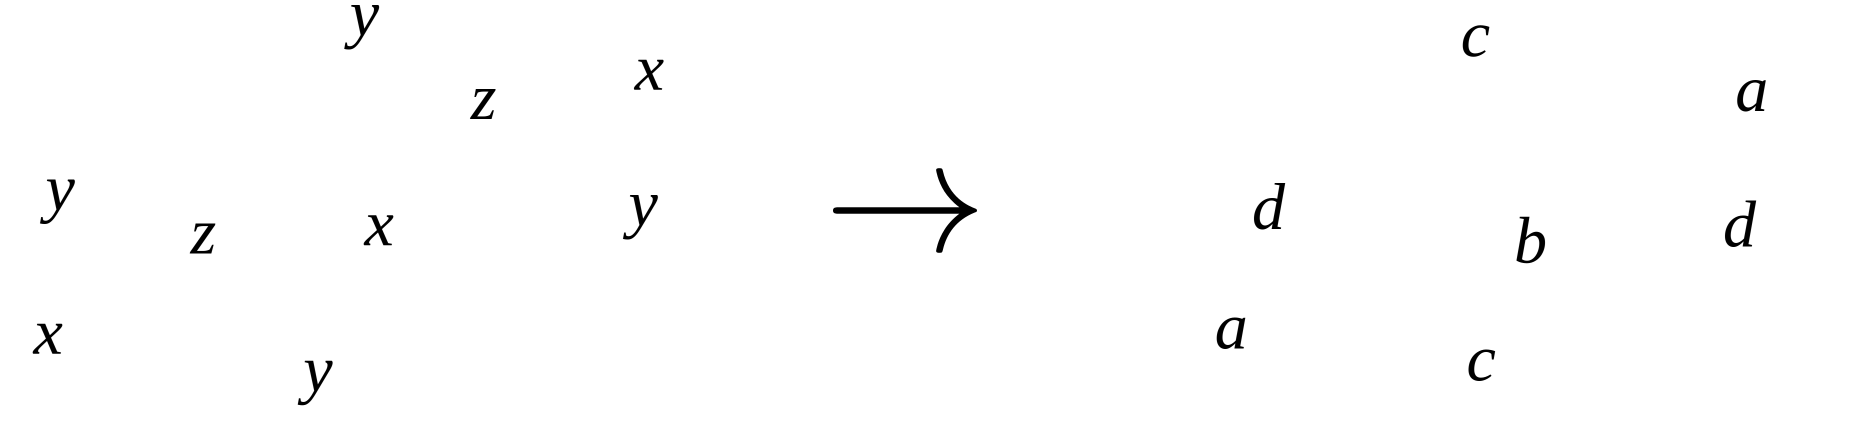
\includegraphics[width=\linewidth]{./appendixLoopModels/hyperhoneycombeffective.pdf}
	\caption{Transition from lattice (10,3)b to effective lattice.}
	\label{fig:appendix1_HyperhoneycombEffectiveLattice}
\end{figure}
%
In the lattice of effective spins, there are four distinct loops of length 6 per unit cell (see Figure~\ref{fig:appendix1_10_3b}).
These four loops taken together form two closed surfaces.
One can show that, for each surface, the product of the four corresponding loop operators is the identity operator, leading to a so-called {\it surface constraint}.
Since the product of these four operators must be the identity, the product of their eigenvalues must be unity.
Thus, there can only be an even number of such loop operators taking eigenvalue $-1$.

From Eq.~\eqref{eq:10_3b_Heff}, one sees that each term in the effective Hamiltonian may be minimized individually by all loop operators taking eigenvalues $+1$.
Since this configuration of loop-operator eigenvalues satisfies all other constraints, one can see that the ground state $\ket{\Psi}$ satisfies $B_p \ket{\Psi} = + \ket{\Psi}$, for all plaquettes $p$.
Furthermore, since
%
\begin{equation}
	B_p = \Upsilon\dag W_p \Upsilon
\end{equation}
%
for all plaquettes $p$, where $W_p$ corresponds to the loop operators defined for the original lattice in the main text, this assignment corresponds to the flux-free sector given by Lieb's theorem~\cite{LiebHPA1992,LiebDMJ1993,LiebPRL1994}.


%
%
%%%%%%%%%%%%%%%%%%%%%%%%%%%%%%%%%%%%%%%%%%%%%%%%%%%%%%%%%%%%%%%%%%%%%%%%%%%%%%%%%%%%%%%%
\section{Lattice (10,3)a}
\label{appendix:LoopModels_10_3a}
%%%%%%%%%%%%%%%%%%%%%%%%%%%%%%%%%%%%%%%%%%%%%%%%%%%%%%%%%%%%%%%%%%%%%%%%%%%%%%%%%%%%%%%%
%
%
%%%%%%%%%%%%%%%%%%%%%%%%%%%%%%%%%%%%%%%%%%%%%%%%%%%%%%%%%%%%%%%%%%%%%%%%%%%%%%%%%%%%%%%%
\subsubsection{Effective Hamiltonian}
%%%%%%%%%%%%%%%%%%%%%%%%%%%%%%%%%%%%%%%%%%%%%%%%%%%%%%%%%%%%%%%%%%%%%%%%%%%%%%%%%%%%%%%%
%
%
As before, all odd-order contributions to the self-energy vanish as they map to states outside of the ground state subspace.
While there are non-zero contributions to the self-energy which are proportional to the identity operator at second and fourth order, the first non-trivial contribution arrives at sixth order in perturbation theory.

The lattice (10,3)a is composed entirely of loops of length 10.
There are four such loops per unit cell which involve six effective spins and either four $x$-bonds and two $y$-bonds (see Figure~\ref{fig:appendix1_10_3a}~(a)) or two $x$-bonds and four $y$-bonds (see Figure~\ref{fig:appendix1_10_3a}~(b)).
Additionally, there are two more loops of length 10 per unit cell which involve \textit{eight} effective spins, four $x$-bonds and four $y$-bonds (see Figure~\ref{fig:appendix1_10_3a}~(c)).

Each of the four plaquettes with six effective spins corresponds to $6! = 720$ terms, each of which is proportional to a loop operator which acts on the effective spins as described in Eq.~\eqref{eq:appendix1_SpinRules}.
The effective Hamiltonian at sixth order in perturbation theory is
%
\begin{equation}
	H_{\rm eff} = {\rm const} + \frac{7 J_x^4 J_y^2}{256 J_z^5} \sum_{p} B^6_p + \frac{7 J_x^2 J_y^4}{256 J_z^5} \sum_{p'} B_{p'}^6,
	\label{eq:10_3a_Heff}
\end{equation}
%
where the first summation is over plaquettes of type $B_1^6$ and $B_2^6$ (see Figure~\ref{fig:appendix1_10_3a}~(a)) and the latter summation is over plaquettes of type $B_3^6$ and $B_4^6$ (see Figure~\ref{fig:appendix1_10_3a}~(b)).
At eighth order, one finds a contribution of
%
\begin{equation}
	\Sigma^{(8)} = {\rm const} + C_6^{(8)} \sum_p B_p^6 + C_6'^{(8)} \sum_{p'} B_{p'}^6 - \frac{5 J_x^4 J_y^4}{2048 J_z^7} \sum_p B_p^8,
	\label{eq:10_3a_SE8}
\end{equation}
%
where $C_6^{(8)}$ and $C_6'^{(8)}$ are eighth-order corrections to the energies of loops of length 6.
%
\begin{figure}[tb]
	\centering
	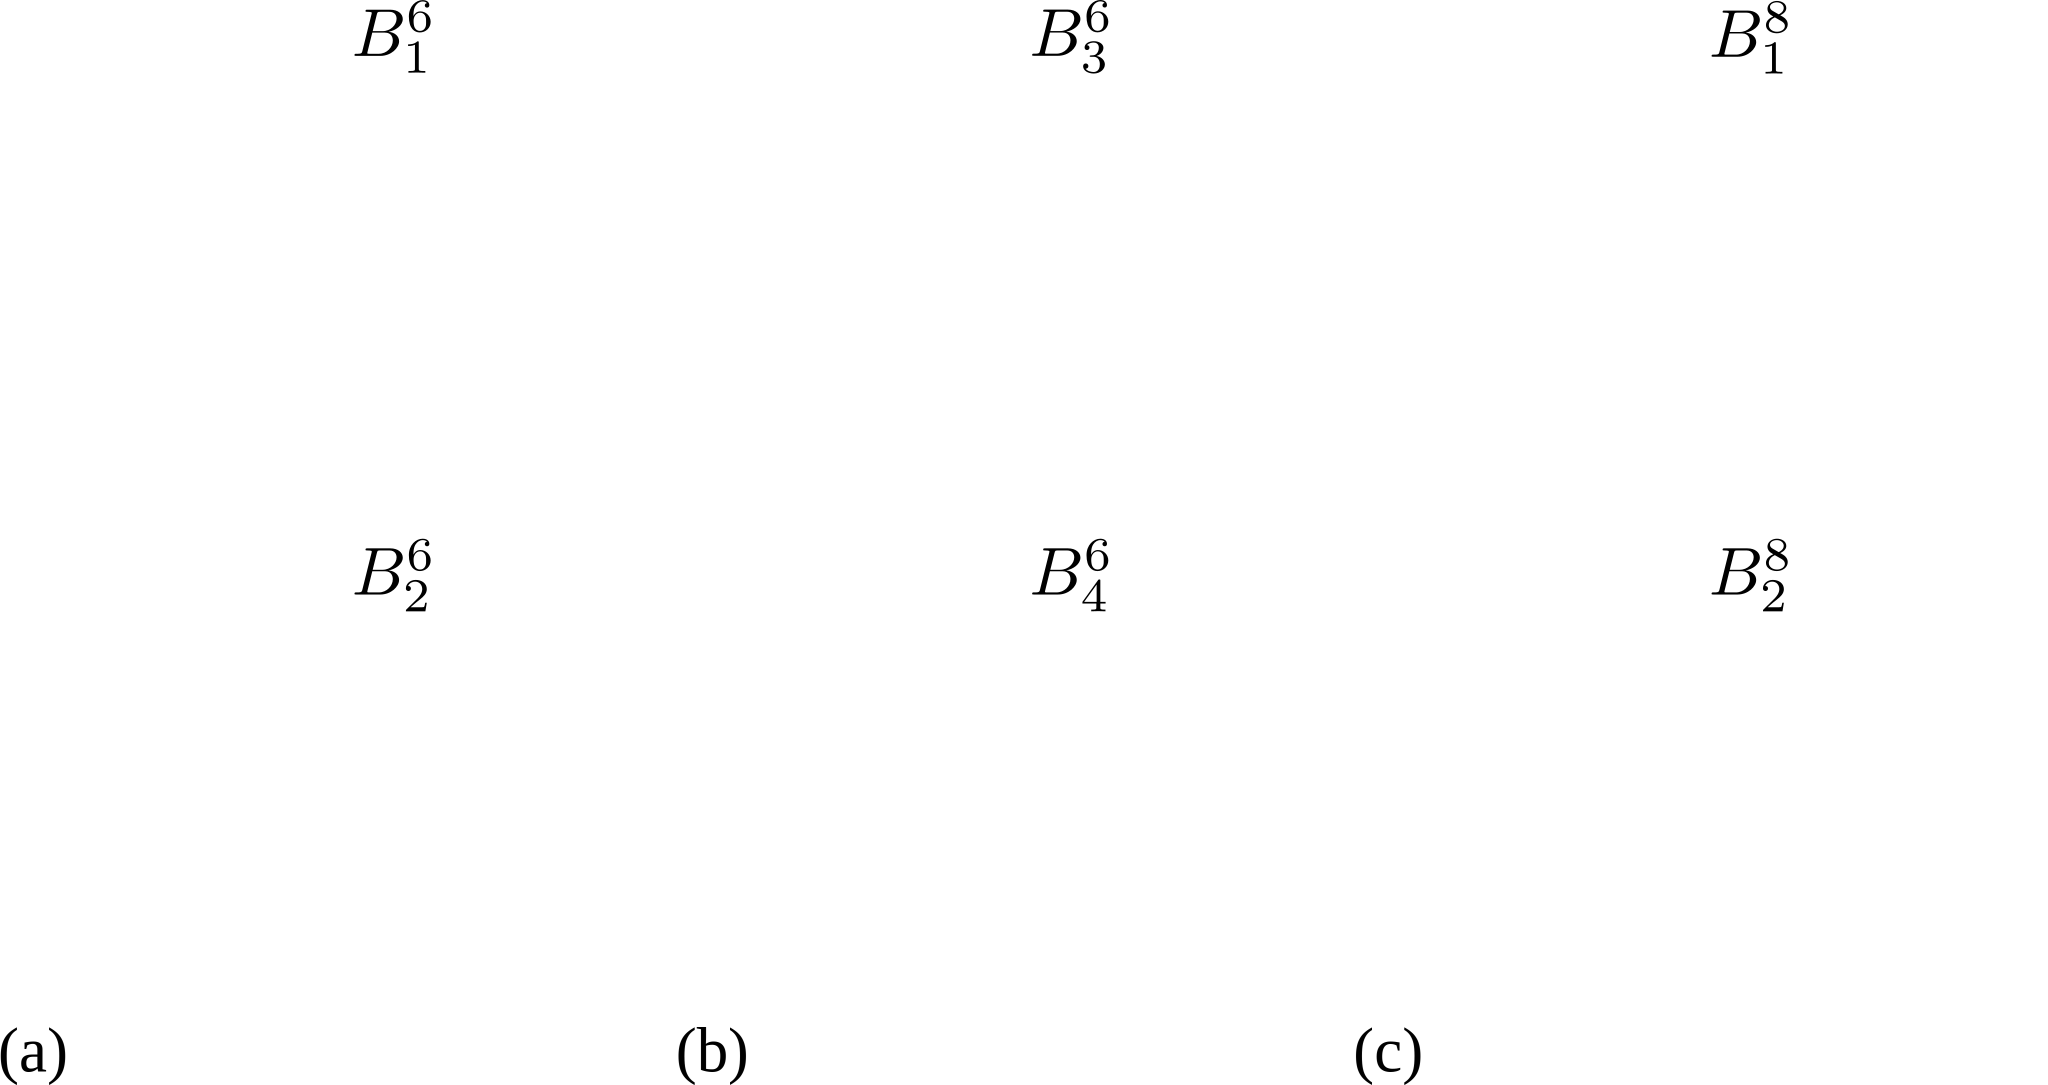
\includegraphics[width=\linewidth]{./appendixLoopModels/10_3a.pdf}
	\caption{Six loops of length 10 in lattice (10,3)a become (a)-(b) four loops of length 6 and (c) two loops of length 8 in the lattice of effective spins.}
	\label{fig:appendix1_10_3a}
\end{figure}
%


%
%
%%%%%%%%%%%%%%%%%%%%%%%%%%%%%%%%%%%%%%%%%%%%%%%%%%%%%%%%%%%%%%%%%%%%%%%%%%%%%%%%%%%%%%%%
\subsubsection{Constraints and the ground state}
%%%%%%%%%%%%%%%%%%%%%%%%%%%%%%%%%%%%%%%%%%%%%%%%%%%%%%%%%%%%%%%%%%%%%%%%%%%%%%%%%%%%%%%%
%
%
In the lattice of effective spins, there are four distinct loops of length 6 per unit cell.
These four loops taken together form two closed surfaces.
One can show that, for each of these surfaces, the product of the four corresponding loop operators is the identity operator, leading to a surface constraint.
Since the product of these four operators must be the identity, the product of their eigenvalues must be unity.
Thus, there can only be an even number of such loop operators taking eigenvalue $-1$.

Additionally, one may consider closed surfaces composed of two loops of length 6 and one of length 8.
Such a product of loop operators again leads to the constraint that the product of all eigenvalues must be unity.
However, since these loop operators of length 8 can be constructed as the product of two loops operators of length 6, this is identical to the surface constraint involving four loop operators of length 6.

From Eqs.~\eqref{eq:10_3a_Heff} and~\eqref{eq:10_3a_SE8}, one sees that each term in the effective Hamiltonian may be minimized individually by all loop operators of length 6 taking eigenvalues $-1$ and all loop operators of length 8 taking eigenvalues $+1$.
Since this configuration of loop-operator eigenvalues satisfies all other constraints, one can see that the ground state $\ket{\Psi}$ satisfies $B_p^6 \ket{\Psi} = -\ket{\Psi}$ for all plaquettes of length 6.
Note that this automatically means $B_p^8 \ket{\Psi} = +\ket{\Psi}$.
Furthermore, since
%
\begin{equation}
	B_p^6 = -\Upsilon\dag W_p^{10} \Upsilon \qquad{\rm and}\qquad B_p^8 = \Upsilon\dag W_p^{10} \Upsilon,
\end{equation}
%
this assignment corresponds to the flux-free sector corresponding to Lieb's theorem of the original model.


%
%
%%%%%%%%%%%%%%%%%%%%%%%%%%%%%%%%%%%%%%%%%%%%%%%%%%%%%%%%%%%%%%%%%%%%%%%%%%%%%%%%%%%%%%%%
\section{Lattice (8,3)b}
\label{appendix:LoopModels_8_3b}
%%%%%%%%%%%%%%%%%%%%%%%%%%%%%%%%%%%%%%%%%%%%%%%%%%%%%%%%%%%%%%%%%%%%%%%%%%%%%%%%%%%%%%%%
%
%
%%%%%%%%%%%%%%%%%%%%%%%%%%%%%%%%%%%%%%%%%%%%%%%%%%%%%%%%%%%%%%%%%%%%%%%%%%%%%%%%%%%%%%%%
\subsubsection{Effective Hamiltonian}
%%%%%%%%%%%%%%%%%%%%%%%%%%%%%%%%%%%%%%%%%%%%%%%%%%%%%%%%%%%%%%%%%%%%%%%%%%%%%%%%%%%%%%%%
%
%
For the lattice (8,3)b, all odd-order contributions to the self-energy vanish while second-order contributions are proportional to the identity.
Non-trivial terms appear at fourth-, sixth- and eighth-orders of perturbation theory.
The lattice (8,3)b contains three loops of length 8 and one loop of length 12 per unit cell (see Figure~\ref{fig:8_3b}).
One of the loops of length 8 involves four effective spins, two $x$-bonds and two $y$-bonds.
The remaining two loops of length 8 involve six effective spins and either two $x$-bonds and four $y$-bonds or four $x$-bonds and two $y$-bonds.
The loop of length 12 involves eight effective spins, four $x$-bonds and four $y$-bonds.

The effective Hamiltonian at fourth-, sixth- and eighth-orders are given by
%
\begin{equation}
\begin{matrix*}[l]
H^{(4)}_{\rm eff} = {\rm const} - \frac{5 J_x^2 J_y^2}{16 J_z^3} \sum_{p} B^4_p, \\
\\
H^{(6)}_{\rm eff} = {\rm const} + \left(-\frac{5 J_x^2 J_y^2}{16 J_z^3} + C_4^{(6)}\right) \sum_{p} B^4_p - \frac{3 J_x^2 J_y^4}{256 J_z^5} \sum_{p} B^6_p - \frac{3 J_x^4 J_y^2}{256 J_z^5} \sum_{p'} B^6_{p'} \\
\\
H^{(8)}_{\rm eff} = {\rm const} + \left(-\frac{5 J_x^2 J_y^2}{16 J_z^3} + C_4^{(6)} + C_4^{(8)}\right) \sum_{p} B^4_p + \left(-\frac{3 J_x^2 J_y^4}{256 J_z^5} + C_{6}^{(8)}\right) \sum_{p} B^6_p + \\
\\
\qquad \left(-\frac{3 J_x^4 J_y^2}{256 J_z^5} + C_{6}'^{(8)}\right) \sum_{p'} B^6_{p'} - \frac{9 J_x^4 J_y^4}{2048 J_z^7} \sum_p B^8_{p},
\end{matrix*}
\label{eq:8_3b_Heff}
\end{equation}
%
where the $C$'s correspond to higher-order corrections to the leading-order loop energies.
%
\begin{figure}[tb]
	\centering
	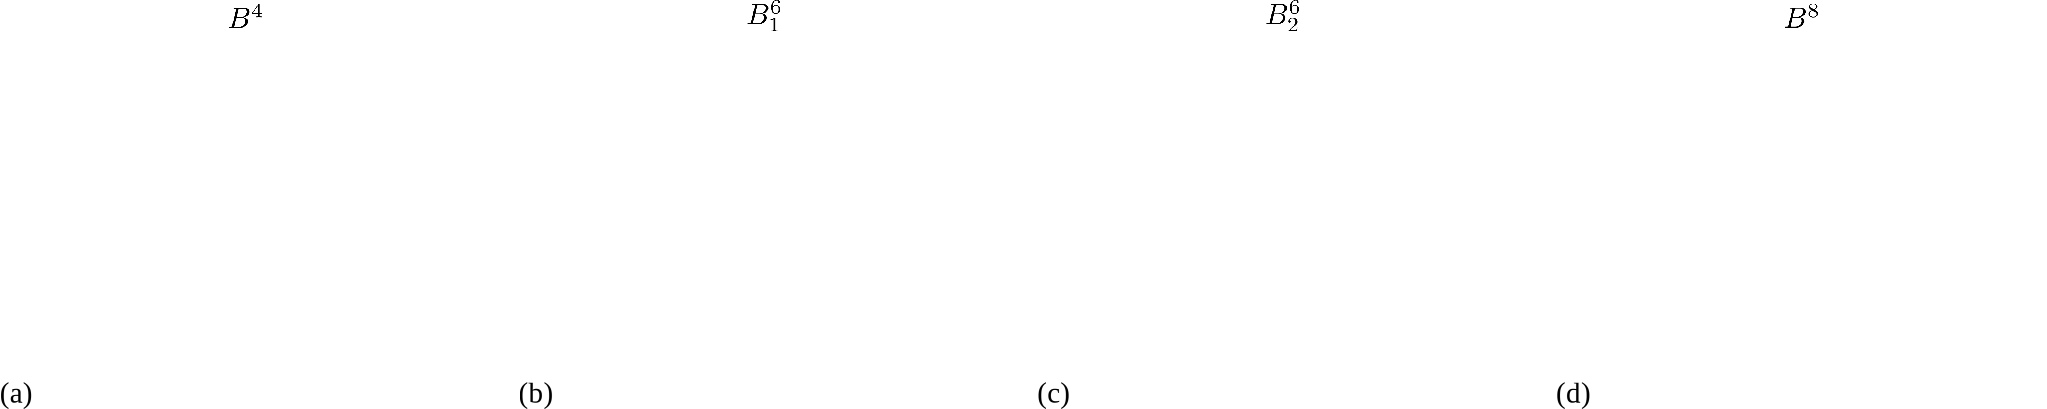
\includegraphics[width=\linewidth]{./appendixLoopModels/8_3b.pdf}
	\caption{Three loops of length 8 in lattice (8,3)b become (a) one loop of length 4, (b)-(c) and two loops of length 6 in the lattice of effective spins. (c) One loop of length 12 becomes a loop of length 8 in the lattice of effective spins.}
	\label{fig:8_3b}
\end{figure}
%


%
%
%%%%%%%%%%%%%%%%%%%%%%%%%%%%%%%%%%%%%%%%%%%%%%%%%%%%%%%%%%%%%%%%%%%%%%%%%%%%%%%%%%%%%%%%
\subsubsection{Constraints and the ground state}
%%%%%%%%%%%%%%%%%%%%%%%%%%%%%%%%%%%%%%%%%%%%%%%%%%%%%%%%%%%%%%%%%%%%%%%%%%%%%%%%%%%%%%%%
%
%
In the lattice of effective spins, there is one loop of length 4, two loops of length 6, and one loop of length 8 per unit cell.
One can form a single closed surface by combining two copies of each loop, where the copies are separated by lattice vectors.
The product of the corresponding loop operators equals the identity operator, leading to a surface constraint.
Since the product of these loop operators must be the identity, the product of their eigenvalues must be unity.
Thus, there can only be an even number of such loop operators taking eigenvalues $-1$.

From Eq.~\eqref{eq:8_3b_Heff}, one sees that each term in the effective Hamiltonian may be minimized by all loop operators taking eigenvalues $+1$.
Since this configuration of loop-operator eigenvalues satisfies all other constraints, one can see that the ground state $\ket{\Psi}$ satisfies $B_p \ket{\Psi} = +\ket{\Psi}$ for all plaquettes $p$.
Furthermore, since 
%
\begin{equation}
	B_p = -\Upsilon\dag W_p \Upsilon
\end{equation}
%
for all plaquettes $p$, this assignment corresponds to the $\pi$-flux sector corresponding to Lieb's theorem of the original model.


%
%
%%%%%%%%%%%%%%%%%%%%%%%%%%%%%%%%%%%%%%%%%%%%%%%%%%%%%%%%%%%%%%%%%%%%%%%%%%%%%%%%%%%%%%%%
\section{Lattice (8,3)c}
\label{appendix:LoopModels_8_3c}
%%%%%%%%%%%%%%%%%%%%%%%%%%%%%%%%%%%%%%%%%%%%%%%%%%%%%%%%%%%%%%%%%%%%%%%%%%%%%%%%%%%%%%%%
%
%
%%%%%%%%%%%%%%%%%%%%%%%%%%%%%%%%%%%%%%%%%%%%%%%%%%%%%%%%%%%%%%%%%%%%%%%%%%%%%%%%%%%%%%%%
\subsubsection{Effective Hamiltonian}
%%%%%%%%%%%%%%%%%%%%%%%%%%%%%%%%%%%%%%%%%%%%%%%%%%%%%%%%%%%%%%%%%%%%%%%%%%%%%%%%%%%%%%%%
%
%
For the lattice (8,3)c, first- and third-order contributions to the self-energy vanish while second- and fourth-order contributions are proportional to the identity.
Non-trivial terms appear at fifth and sixth order in perturbation theory.
The lattice (8,3)c contains six loops of length 8 per unit cell.
Four of these loops contain five effective spins (see Figures~\ref{fig:appendix1_8_3c}~(a)-(d)).
The first two contain three $x$-bonds and two $y$-bonds while the other two contain two $x$-bonds and three $y$-bonds.
The remaining two loops contain six effective spins, three $x$-bonds and three $y$-bonds (see Figures~\ref{fig:appendix1_8_3c}~(e) and (f)).
At sixth order, the effective Hamiltonian reads
%
\begin{equation}
H_{\rm eff} = {\rm const} + \frac{5 J_x^3 J_y^2}{128 J_z^4} \sum_{p} B^5_p - \frac{5 J_x^2 J_y^3}{128 J_z^4} \sum_{p'} B^5_{p'} - \frac{3 J_x^3 J_y^3}{256 J_z^5} \sum_{p} B^6_{p},
\label{eq:8_3c_Heff}
\end{equation}
%
where the first summation is over plaquettes of type $B^5_1$ and $B^5_2$, the second summation is over plaquettes of type $B^5_3$ and $B^5_4$, and the third summation is over plaquettes of type $B^6_1$ and $B^6_2$ (see Figure~\ref{fig:appendix1_8_3c}).

%
\begin{figure}[tb]
	\centering
	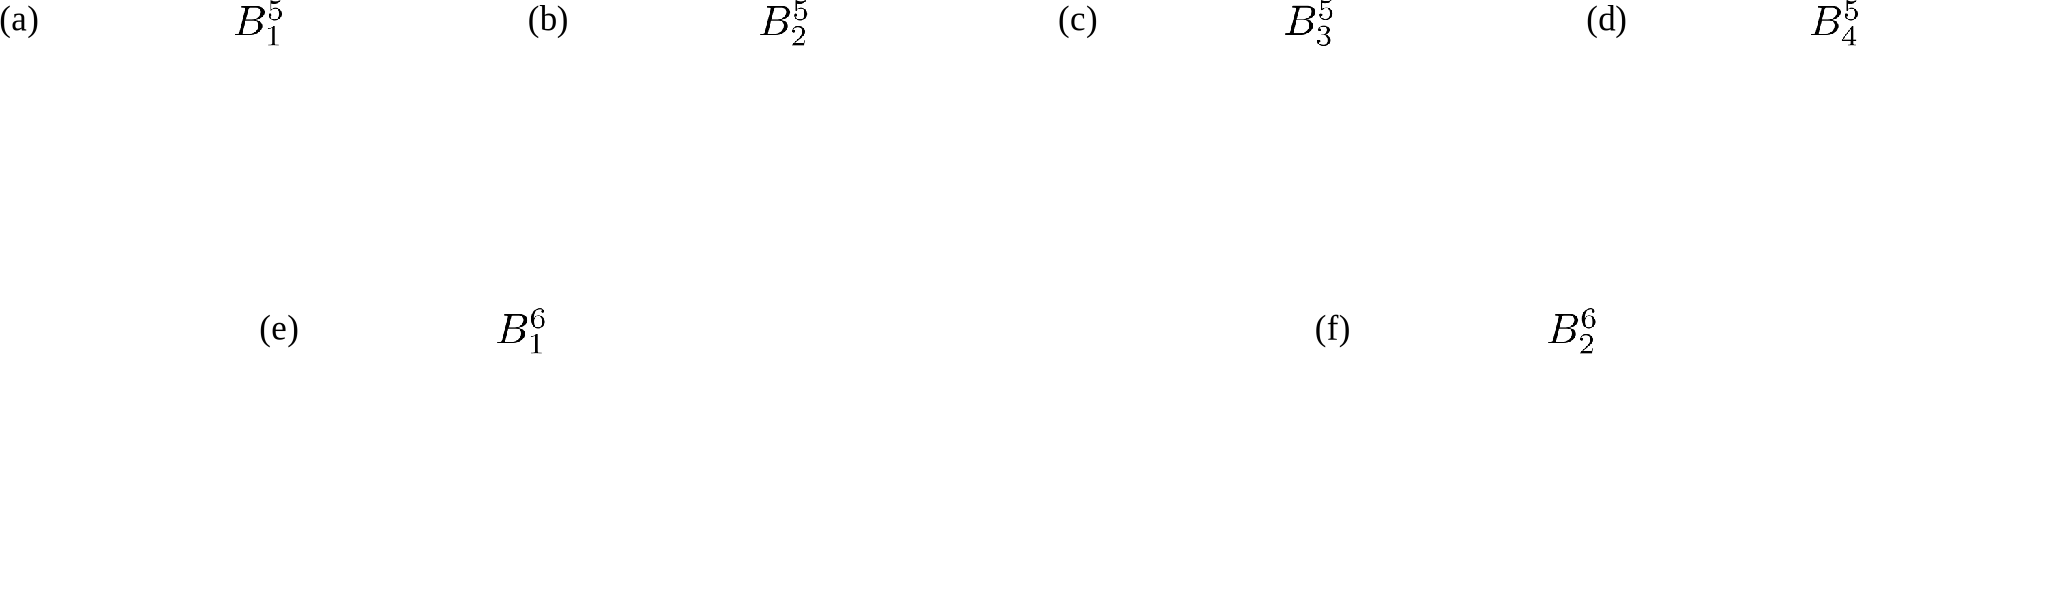
\includegraphics[width=\linewidth]{./appendixLoopModels/8_3c.pdf}
	\caption{Six loops of length 8 in lattice (8,3)c become (a)-(d) four loops of length 5 and (e)-(f) two loops of length 6 in the lattice of effective spins.}
	\label{fig:appendix1_8_3c}
\end{figure}
%


%
%
\subsubsection{Constraints and the ground state}
%
%
In the lattice of effective spins, there are four distinct loops of length 5 per unit cell and two of length 6 per unit cell.
One can form two closed surfaces by combining either the loops corresponding to $B_1^5$, $B_3^5$ and $B_1^6$ or the loops corresponding to $B_2^5$, $B_4^5$ and $B_2^6$.
The product of the corresponding loop operators equals the identity operator for both surfaces, leading to two surface constraints.
Since the product of these loop operators must be the identity, the product of their eigenvalues must be unity.
Thus, there can only be an even number of such loop operators taking eigenvalue $-1$.

From Eq.~\eqref{eq:8_3c_Heff}, one sees that each term in the effective Hamiltonian may be minimized by all loop operators of the form $B_1^5$ or $B_2^5$ taking eigenvalues $-1$, all loop operators of the form $B_3^5$ or $B_4^5$ taking eigenvalues $+1$, and all loop operators of length 6 taking eigenvalues $+1$.
However, such an assignment of loop-operator eigenvalues is incompatible with the surface constraints described above.
The least energetically costly move is to take the loop operators of length 6 to have eigenvalues $-1$ rather than $+1$.
Thus, the ground state $\ket{\Psi}$ satisfies $B_p^5 \ket{\Psi} = -\ket{\Psi}$ for $p=1$ or $2$, $B_p^5 \ket{\Psi} = +\ket{\Psi}$ for $p=3$ or $4$, and $B_p^6 \ket{\Psi} = -\ket{\Psi}$.
Furthermore, since
%
\begin{align}
B_{1,2}^5 = \Upsilon\dag W_{1,2}^8 \Upsilon, \qquad
B_{3,4}^5 = -\Upsilon\dag W_{3,4}^8 \Upsilon, \qquad{\rm and}\qquad
B_{1,2}^6 = - \Upsilon\dag W_{5,6}^8 \Upsilon,
\end{align}
%
this assignment corresponds to $W_{1,2}^8 = -1$, $W_{3,4}^8 = -1$ and $W_{5,6}^8 = +1$.
Indeed, this flux sector was found to be the ground state for sufficiently strong $J_z$ in a subsequent quantum Monte Carlo study~\cite{EschmannPRL2019}.